\documentclass[a4paper, 10pt]{article}
\usepackage{geometry}
\geometry{left=3cm,right=3cm,top=3cm,bottom=3cm}
\usepackage{footmisc}
\usepackage[UTF8]{ctex}
\usepackage{subfigure}
\usepackage[graphicx]{realboxes}
\begin{document}

  \title{{\huge \textbf {浅谈新能源汽车出海}}
  
  {\LARGE -从行业分析角度窥探中国经济未来的着力点}}
  \author{郑志恒  2300012559  物理学院\\ 黎锦添  2300012562  地球与空间科学学院}
  \date{}
  
  \maketitle
  \section{摘要}
  当前,世界经济正处于下行周期。基于此,部分国家开始采取贸易保护主义政策以提振自身的经济发展。因此,作为制造业大国的中国近年一直面临着出口压力。在这种情况下,中国新能源汽车的出口却与其它产业出口的表现大相径庭。笔者认为,研究这一现象背后的原因对于规划中国未来经济发展的方向意义非凡。因此,笔者结合供求理论、新结构经济学理论、发展型国家理论等经济学理论,对新能源汽车行业出海的成功进行理论分析,并由此阐述笔者对于未来中国经济发展的一些看法。
  
  \vspace{10pt}
  \noindent 关键词:新能源汽车产业、比较优势战略、政府干预、世界市场、发展型国家理论
  \section{正文}
  \subsection{新能源汽车出口的概况 \protect\footnote{此处新能源汽车指纯电、插混、混动三种类型的总和。}}
  \begin{figure}[ht]
    \centering 
    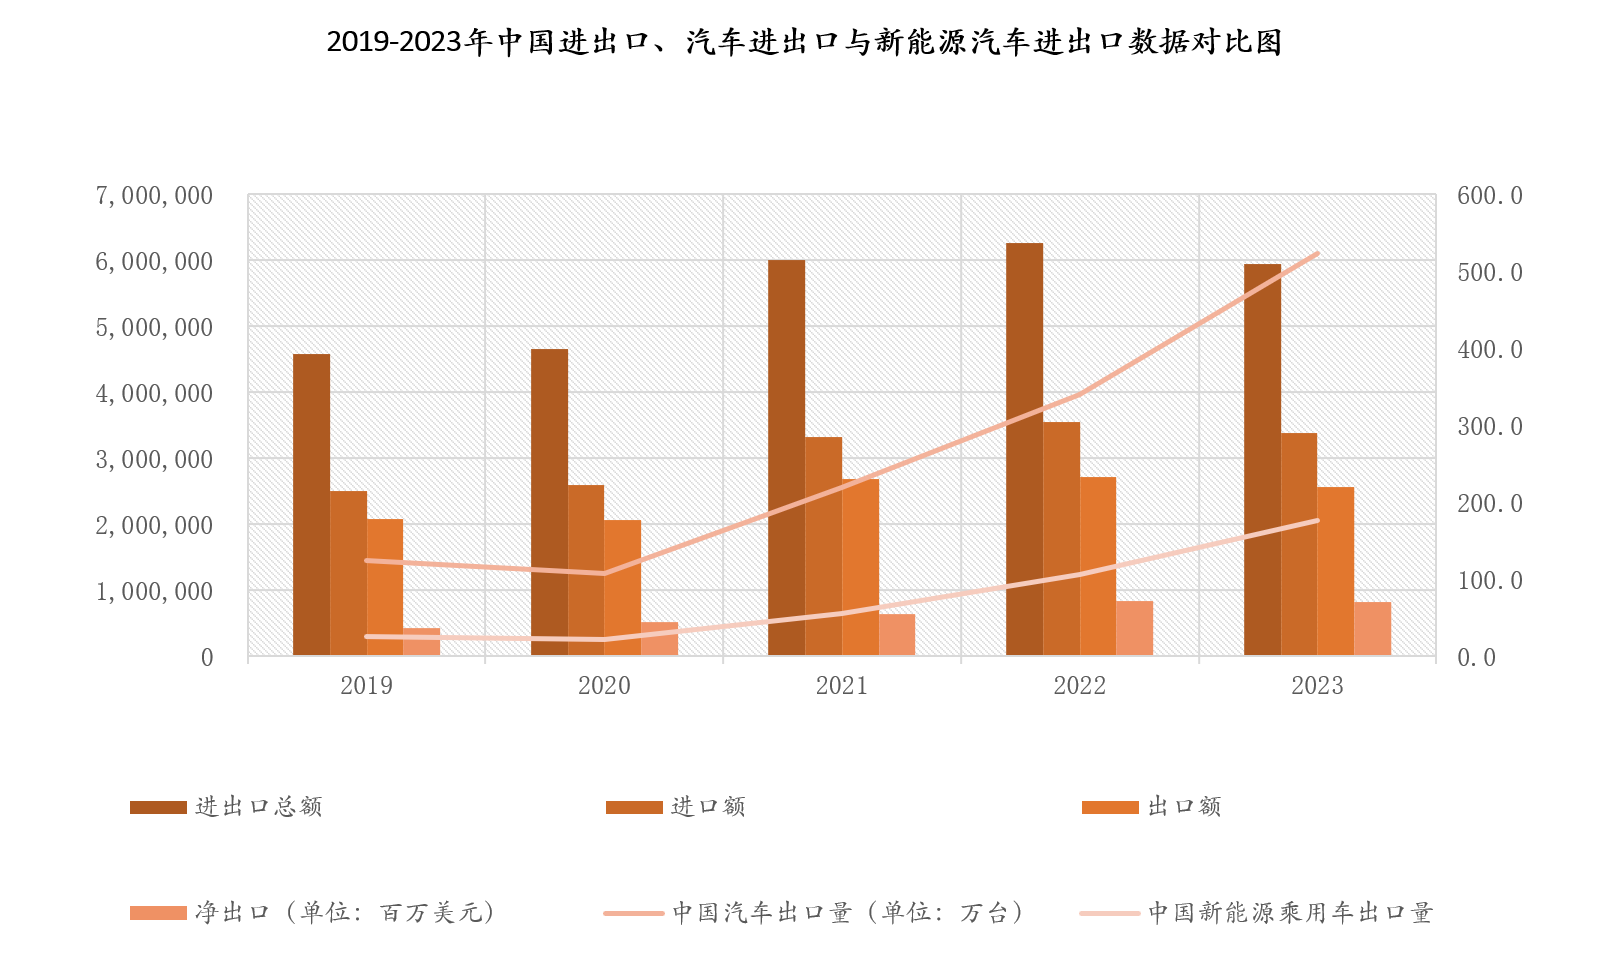
\includegraphics[height=8cm,width=14.5cm]{fg1.png}
    
    \caption{数据来源:国家统计局与中国汽车流通协会}
    \label{1}
    
    \end{figure}
    \begin{figure}[ht]
      \centering 
      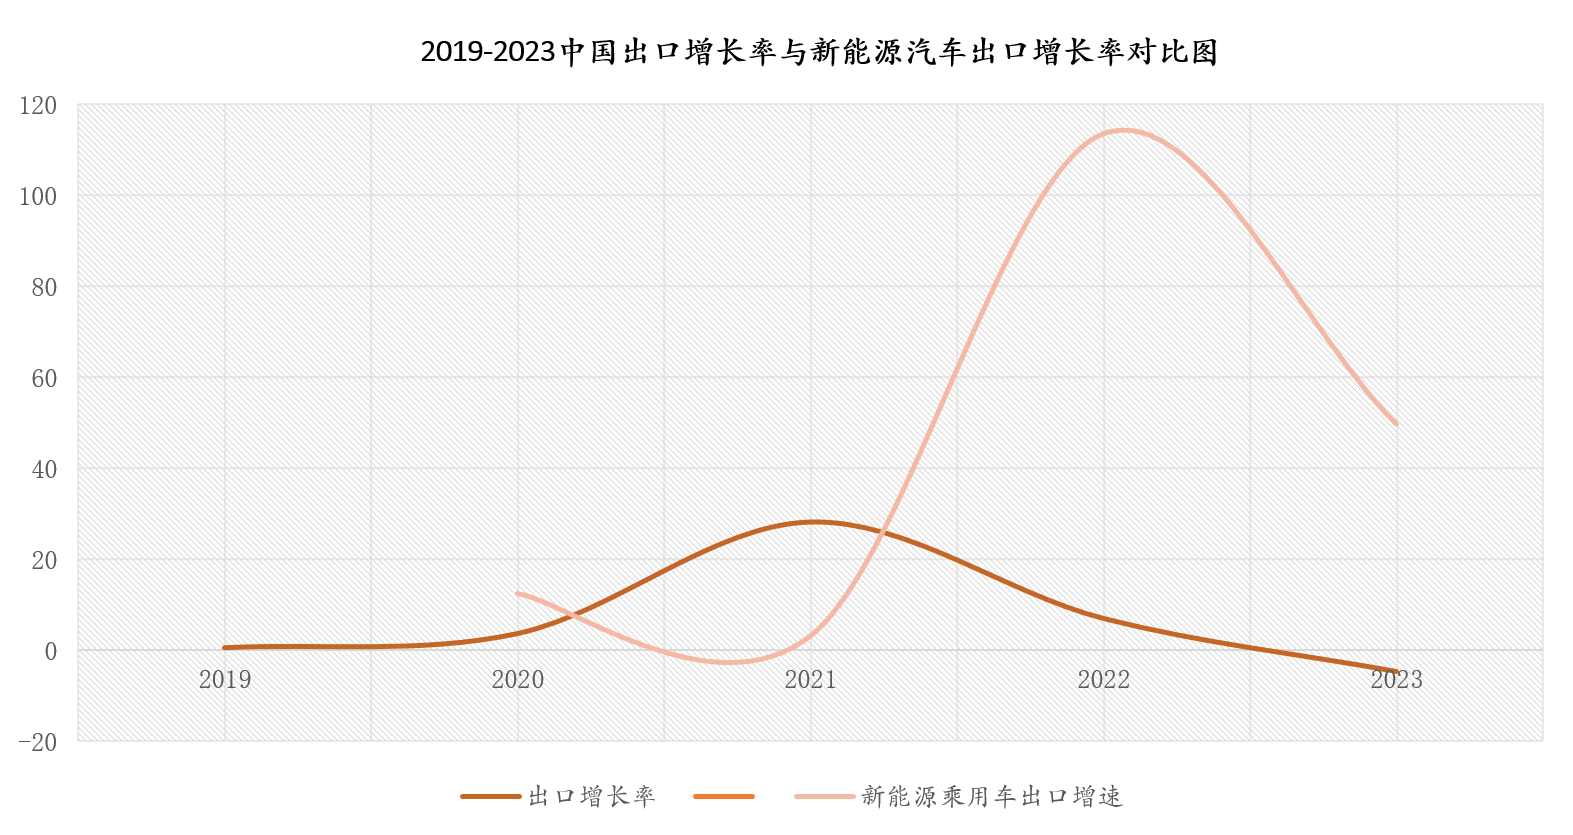
\includegraphics[height=8cm,width=14.5cm]{fg2.png}
      
      \caption{数据来源:国家统计局与中国汽车流通协会}
      \label{2}
      
      \end{figure}
    笔者统计了近五年中国进出口与新能源汽车进出口的绝对值与增长率,由图1与图2可以看出,近五年中国新能源汽车的出口与中国总的进出口呈现出相反的增长趋势。其中,2022年成为中国新能源汽车出海的分水岭,在2022年以前,中国新能源汽车的出口还处于起步探索阶段;2022年以后,新能源汽车的出口开始呈现大额增长,在2024年前8个月,中国新能源车的全球市场份额达到67\%,可以说席卷了世界市场。这一现象完全背离经济下行周期的大环境趋势。

    笔者认为,新能源汽车出海的逆周期增长奇迹是供给侧与需求端共同作用的结果。因此,这些要素也决定了未来新能源汽车出海的发展方向。由此,我们可以探索中国未来经济发展和供给侧改革的模板,从而更好地制定发展战略和产业政策。
\subsection{供给侧分析}
  \subsubsection{技术因素-“有为市场”下技术迭代引发的产业结构转型}
  \begin{figure}[ht]
    \centering 
    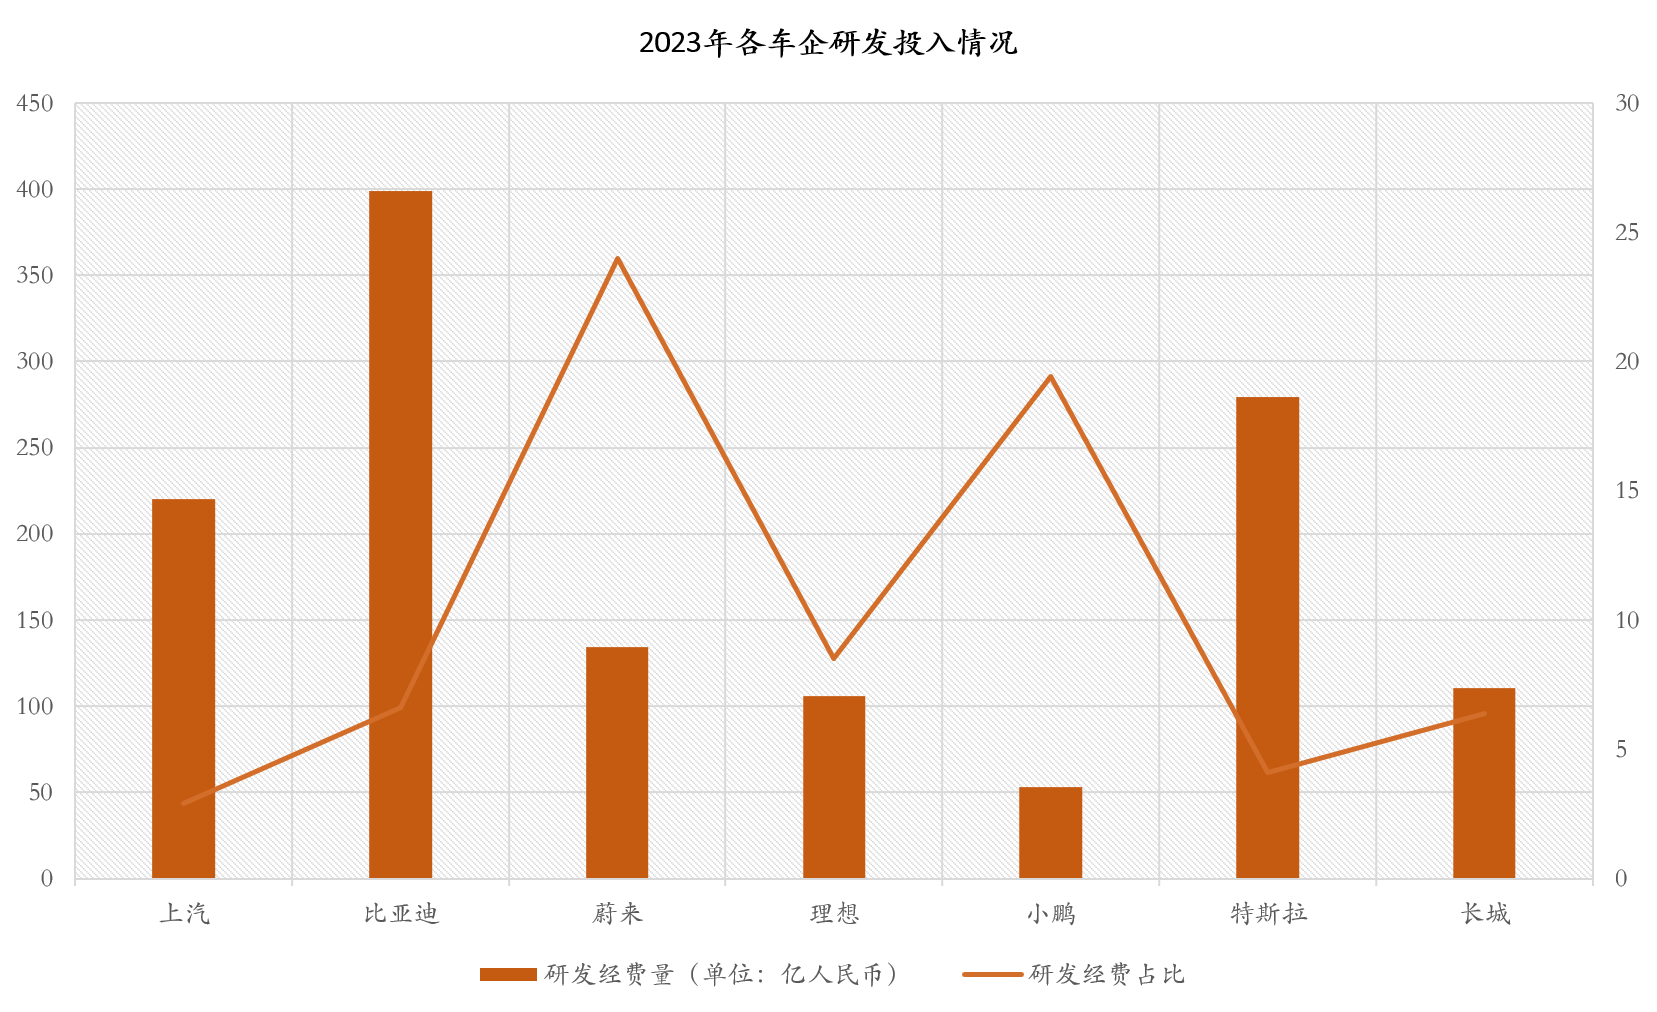
\includegraphics[height=7cm,width=11.5cm]{fg3.png}
    
    \caption{数据来源:公开数据}
    \label{3}
    
    \end{figure}
    \begin{figure}[ht]
      \centering 
      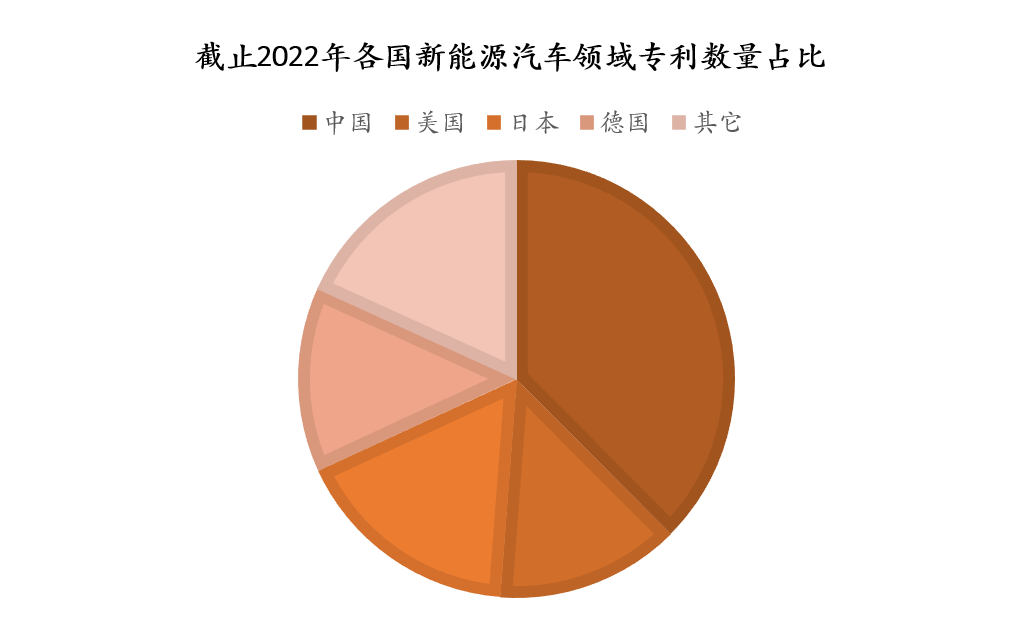
\includegraphics[height=6.3cm,width=10.5cm]{fg4.png}
      
      \caption{数据来源:全球汽车专利大数据平台}
      \label{4}
      
      \end{figure}
    为什么中国的新能源汽车能快速地席卷世界市场,并完成对传统汽车制造业大国的反超?技术的快速完善的发展是关键因素之一。根据公开数据,截止2022年9月,中国在新能源汽车领域的专利公开量占整个领域比重达到了41.2\%。这说明,中国在新能源汽车制造领域已经积累了大量技术优势。在新能源造车的赛道上,中国已经完成了“弯道超车”。
    
    同时,中国新能源车企普遍拥有较高的研发经费占比。传统车企和老牌汽车制造企业如大众、丰田和福特等,一般研发投入占比都在5\%上下,而中国新能源车企的研发占比普遍都在7\%以上,如蔚来、小鹏等新势力车企为了抹平技术差距、追赶技术水平更是拥有高额的研发占比。普遍的高研发经费占比背后的本质是各车企为了占领市场而自发进行的高强度竞争,在结果上体现为技术的快速迭代。
上述分析说明,近年中国在新能源汽车制造的发展绝不是简单的资本要素投入的增加,而是技术迭代引发的产业结构转型。

根据新结构经济学理论,“在任何给定时点, 一个经济体的最优产业结构内生决定于该时点上劳动、资本和自然资源的相对丰裕程度”\footnote{引用自《新结构经济学—重构发展经济学的框架》}。新能源汽车产业目前处于市场开拓阶段,是典型的技术密集型制造产业,且有着庞大的市场需求,是典型的适配中国要素禀赋结构的产业。同时,比较优势战略要求“有为市场”的参与,即依靠市场的竞争机制来驱动企业不断创新,从而带来经济的发展。新能源汽车领域当下的表现也符合这一理论的解释。这具体表现为越来越多的新企业加入新能源汽车制造行业(如小米、蔚来、理想等),与旧有的企业(如比亚迪、特斯拉)进行充分竞争。在国内市场经历充分竞争的车企,积累了充足的技术优势和竞争经验,同时还打造了品牌口碑,在出口时天然地拥有更强的竞争力。这一出口优势是中国的本土燃油车企面对德日的老牌造车企业时所不具备的。

\subsubsection{政策因素-市场扩张下“有为政府”的迅速跟进}
    2023年,商务部印发《关于支持新能源汽车贸易合作健康发展的意见》,为新能源汽车的出海保驾护航。具体表现为鼓励海外研发合作、提升海外售后与合规经营能力、打造国际贸易平台、健全物流运输体系等等。这些举措一定程度上引导车企发展国外的产业链,催动企业的本地化、服务化和合规化。

    可以说,《意见》紧跟行业发展的趋势,是政府对于新能源汽车出海的迅速跟进,完全符合比较优势战略理论为政府规定的责任范围。比较优势战略要求一个公开,竞争,开放的市场,这要求政府在对外贸易平台打造和沟通国内外评级体系以减少信息不对称方面作有效的跟进。除此之外,《意见》还指出要提供信贷与货币跨境结算支持、完善进出口管理机制等,这些举措都旨在打造一个完善的出海体系,为企业减少不必要的成本。

    同时,在补贴方面,政府开始逐渐实行“退坡”政策。这是由于,中国的新能源汽车行业已经开始逐渐走向成熟,补贴政策反而会破坏企业的自生能力,产生政策性负担,不利于行业的发展。事实上,已经存在一部分小型车企出现“补贴依赖”的现象。因此,尽早对补贴政策进行改革十分有必要。

    由此可见,政策干预在新能源汽车的发展和出口上作用巨大。在行业发展的起步阶段,这种作用主要表现为高额的补贴,采用直接手段减少企业开拓市场的成本;在稳定增长期和行业出海方面,这种作用则表现为补贴的“退坡”和“有为政府”。这种角色定位的转换在最大程度扶持行业发展的同时尽力减少对企业的直接干预,保护企业的自生能力,符合比较优势战略的理论。
    \begin{figure}[ht]
      \centering 
      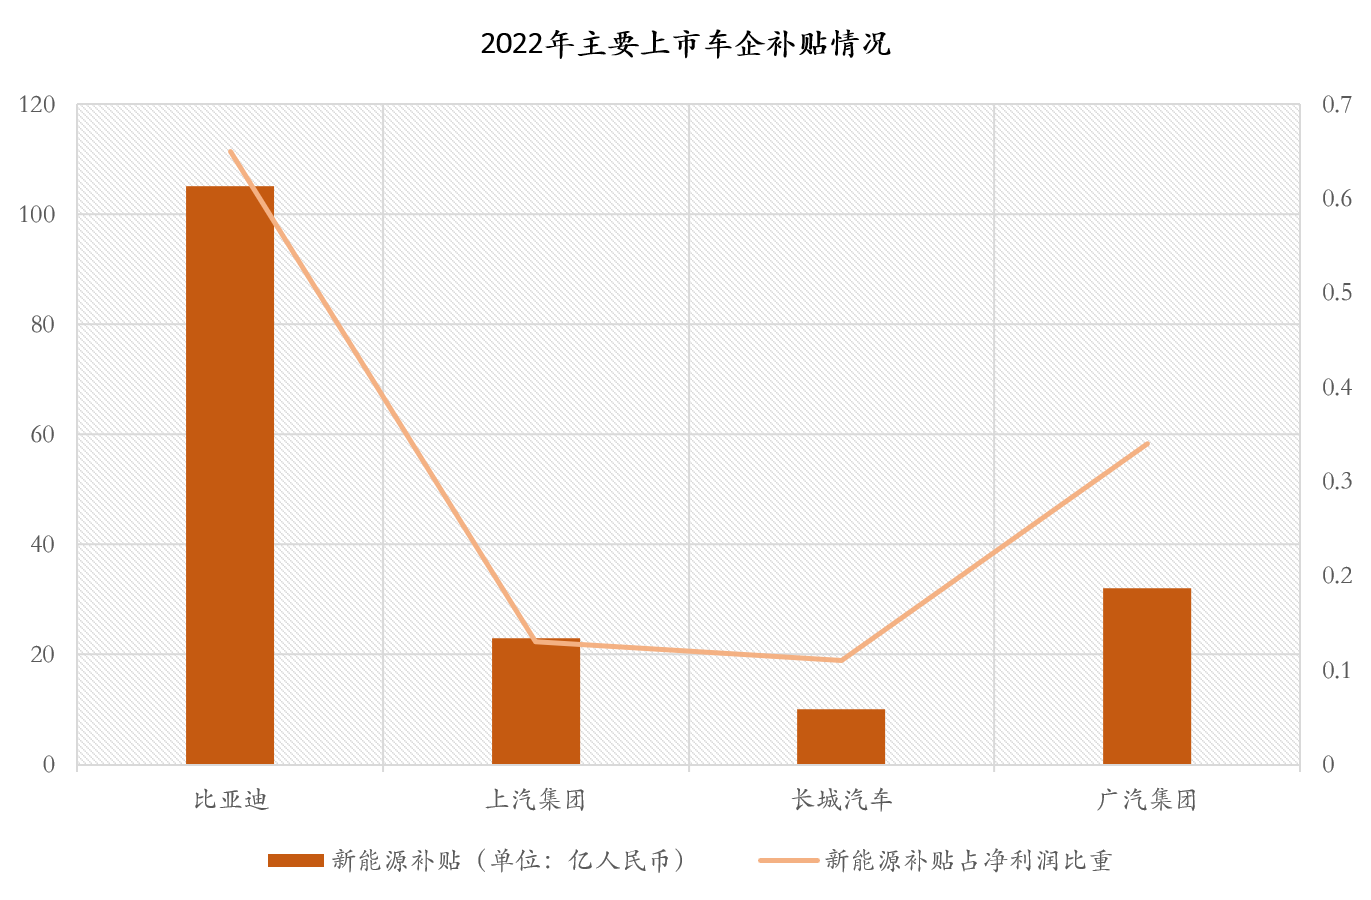
\includegraphics[height=9cm,width=13.5cm]{fg5.png}
      
      \caption{数据来源:公开数据}
      \label{5}
      
      \end{figure}
    \subsection{需求端分析}
    \subsubsection{东南亚市场:积极的政策扶持与较低的贸易壁垒}
\textbf{东南亚以其优越的地理位置和政策红利成为中国新能源车企出海的主要目标市场之一。在东南亚市场,风险与机遇并存。}

    近年来,东南亚国家普遍对新能源汽车采取积极的态度,泰国、印度尼西亚和马来西亚等国陆续提出了电动汽车市场发展的战略目标。而东南亚国家的新能源汽车产业链布局整体较为薄弱,因此,政府为扶持本地产业链,对于进口新能源汽车出台了一系列积极的支持政策,降低贸易壁垒,并支持本土化建厂,以带动本国新能源汽车产业链的建设和发展。
    \begin{figure}[ht]
      \centering 
      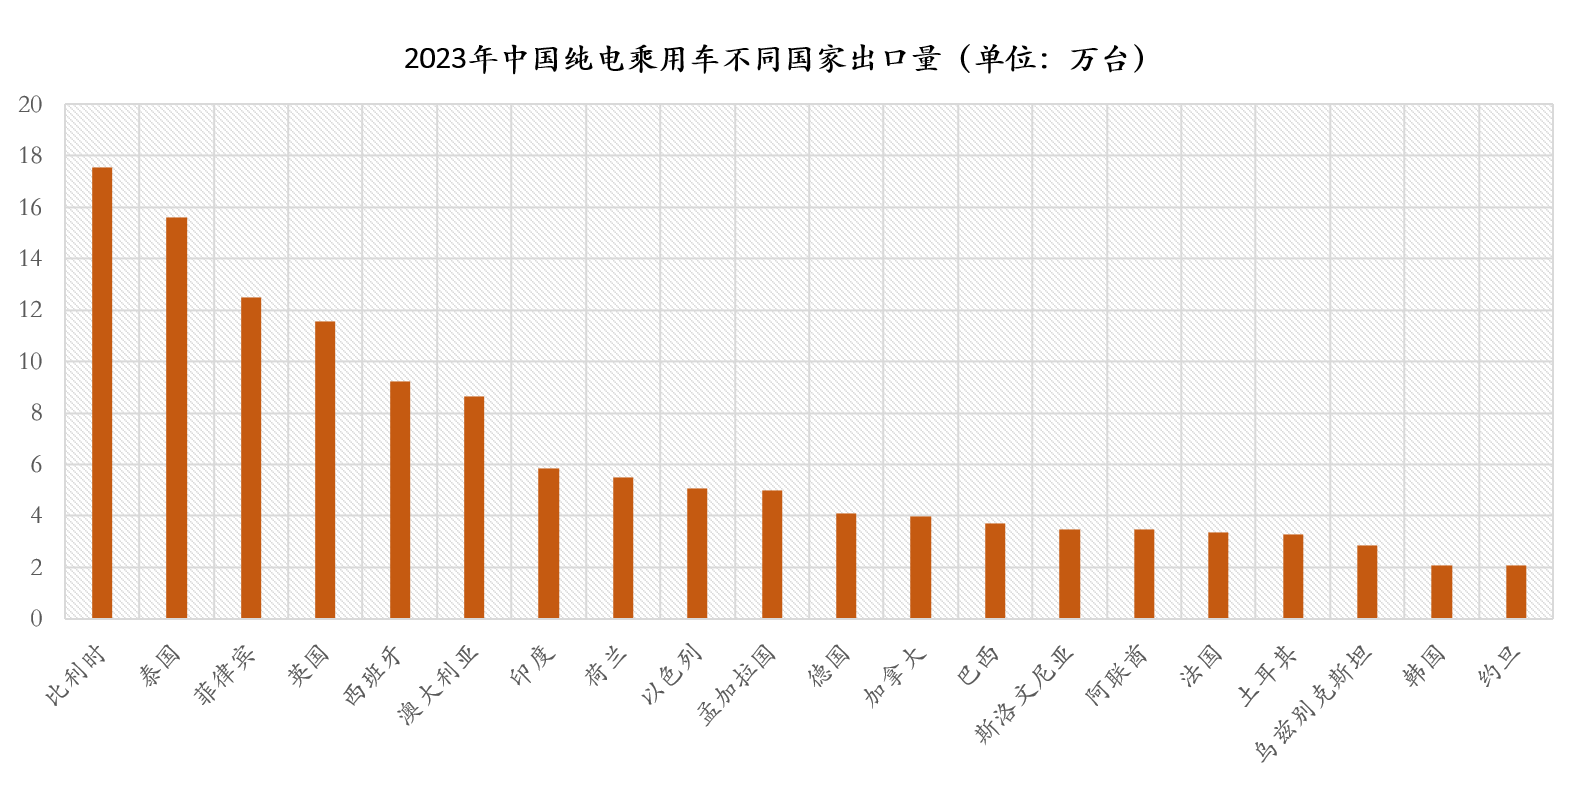
\includegraphics[height=7.0cm,width=13.7cm]{fg6.png}
      
      \caption{数据来源:公开数据}
      \label{6}
      
      \end{figure}
    泰国、印度尼西亚和马来西亚是东南亚新能源汽车渗透率最高的三个国家,其政府都陆续出台了关税减免和财政补贴等鼓励新能源汽车进口的政策。例如,泰国实施消费税减免、购车补贴、整车和关键零部件关税减免,并减免电动汽车供应方企业的企业所得税,供应方企业最高可享8年的免企业所得税优惠;马来西亚还提出在2025年底前对本地组装的电动汽车免征关税。同时,各国积极推动充电桩等配套设施的完善,提出了未来五至十年内充电桩建设的规模目标,并对充电桩生产的相关企业实行政策激励,如泰国对充电桩生产相关企业免征5年关税。这些国家政策的共同点都是降低关税壁垒以及鼓励支持本土化建厂。

    此外,地理位置优势和人口红利带来的消费市场潜力也为中国新能源汽车出口东南亚提供了更多利处。东南亚总人口数量约6亿,其中印度尼西亚和菲律宾人口过亿,分别约2.78亿和1.17亿,且东南亚国家人口老龄化程度较低,人口结构较优,拥有庞大的新能源汽车消费市场潜力。同时,东南亚与中国地理位置距离较近,为运输带来便利。这些优势共同使得东南亚成为中国新能源汽车出口的第三大核心市场,仅次于北美和南美。其中,2023年,泰国是中国纯电乘用车出口量第二大的国家,出口量达到了15.59万台,仅次于比利时。
    


    但值得注意的是,东南亚市场在充满机遇的同时,也为中国新能源汽车企业带来了新的挑战。首先,东南亚国家政府普遍支持本土化建厂,中国企业在建设本土化工厂、适应本土需求等方面存在挑战;其次,东南亚国家的配套基础设施建设和售后服务体系整体上相对不完善,需要中国企业加大对于售后服务体系和设施建设的投入;此外,东南亚部分国家的金融体系和信贷体系较不完善,可能导致新能源汽车的交易出现波动。




    \subsubsection{欧美市场:广阔的市场前景与反补贴税的考验}
    \textbf{欧洲是目前除了中国以外最大的新能源汽车市场。}
    
    根据《欧洲气候法》和《欧洲绿色协议》,欧盟承诺到2030 年,温室气体净排放量将比1990 年至少减少55\%。这一目标意味着欧洲市场对新能源汽车的巨额需求。
    北欧地区汽车工业体系较为落后、西欧地区新能源车产能短缺,
导致欧洲的新能源车供给主要依赖进口。

同时,欧洲部分国家颁布了吸引外资的政策,例如捷克的《投资鼓励法》规定,对包括新能源汽车在内的制造业启动新技术中心和战略服务中
心等投资活动提供支持。支持形式为提供最多10个纳税期(免
税期)的企业所得税减免或现金补贴。类似的政策给全球新能源车企带
来了机遇,对于中国车企来说,欧洲市场既有着巨大的政策红利,又拥有不可估量的市场潜力,是优质的出口市场。也正因如此,以中国车企为代表的各国新能源车企纷纷涌入欧洲,欧洲新能源车销量渗透率从2018年不足3\%增长至
2023年的23\%,势头迅猛。
    由于中国新能源汽车企业在国内市场积累了大量技术优势与竞争经验,国产新能源汽车的出口迅速冲击欧洲市场,市场占有率逐年提高。
    \begin{figure}[ht]
      \centering 
      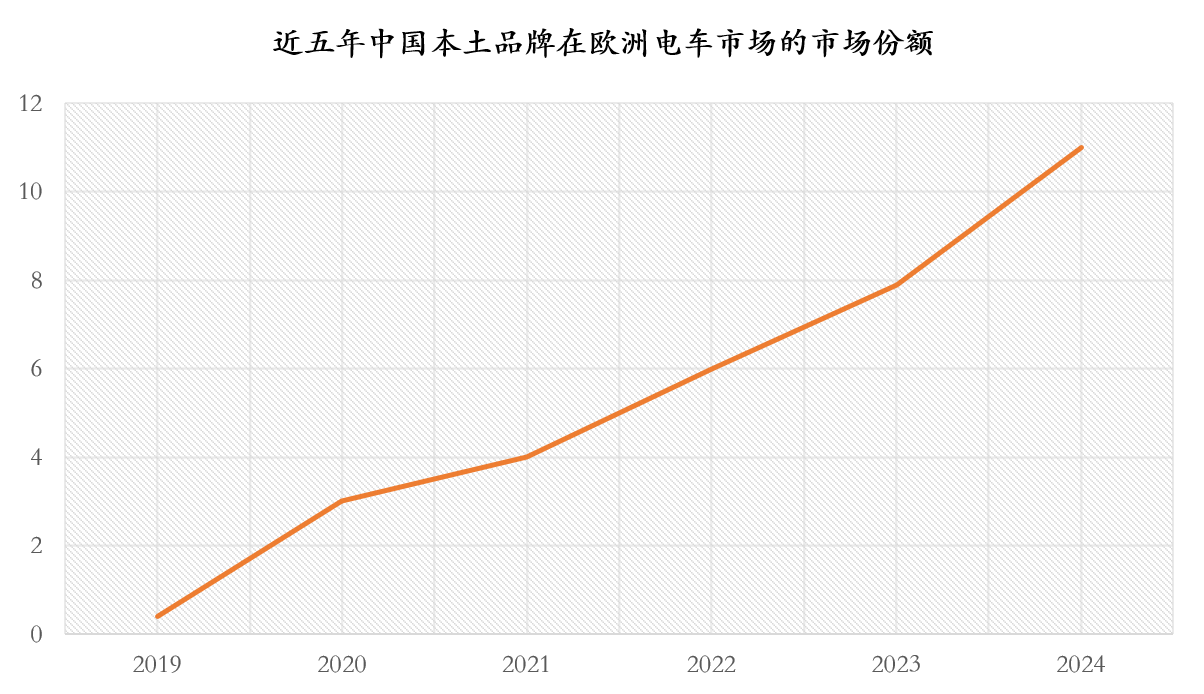
\includegraphics[height=6.5cm,width=11.3cm]{fg7.png}
      
      \caption{数据来源:公开数据 }
      \label{6}
    \end{figure}\footnote{图6未计入中国收购的欧洲品牌电动汽车的市场份额}
    
其中,比利时、西班牙和俄罗斯等国家都是中国新能源汽车的重要市场。中国向比利时出口的汽车中,新能源汽车占比已经达到80.6\%。

    为了应对中国车企对欧美市场的冲击,抢夺市场份额,欧美出台多项政策实行贸易保护。其中包括《净零工业法案》《关键原材料法案》《美国通胀削减法案》等,具体操作主要为:要求一定比例的原材料和生产线在当地进行、对关键原材料和电池组件来自中国的汽车克扣税收抵免等。

    其次,欧洲还提高了关税壁垒,对水泥、电力、化肥、钢铁、铝、
    氢气六种进口产品的隐含排放量进行征税,其既包括生产过程中的直接碳排放,也包括其消耗电力对应的间接碳排放。
    
    除此之外,欧委会认为,“中国企业(包括民营企业)是政府宏观政策和特定目标的实施者,而不是有权独立决策的自由市场参与者”,并在调查后得出结论:“进口自中国的电动汽车的生产商获得了中国国家补贴,并给欧盟电动汽车产业造成了实质性损害威胁。因此欧委会决定对原产于中国的电动汽车征收反补贴税。”\footnote {引用自《对原产于中华人民共和国的电动乘用汽车进口征收临时反补贴税》}
    \vspace{10pt}
    \begin{center}
    \begin{tabular}{|c|c|}
      \hline
      中国电动汽车企业 & 加征关税额\\
      \hline
      比亚迪 & 17\%\\
      \hline
      吉利 & 18.8\%\\
      \hline
      上汽集团 & 35.3\%\\
      \hline
      配合调查但未被单独抽样的中国电动汽车生产商 & 20.7\%\\
      \hline
      中国其它未合作的电动汽车生产商 & 35.3\%\\
      \hline
    \end{tabular}

    \vspace{10pt}

表1\footnote{信息来源:《2024中国新能源汽车出海十大趋势洞察》}

  \end{center}
  \vspace{10pt}
    欧洲的一系列措施会使得中国丢失欧洲市场吗?这对于中国新能源车企提出了挑战。事实上,从宏观的视角来看,中国的制造业出口整体都受到了西方国家的遏制。“贸易战”就是最典型的案例。因此,高关税壁垒、贸易调查和政策限制是许多中国出口产业面临的共性问题。因此,笔者将在后续详细讨论中国企业针对这一问题的对策。
    \subsubsection{小结:宏观视角-世界市场与中国}
    目前,世界市场普遍面临需求疲软的问题,这带来贸易保护主义和逆全球化的趋势,WTO建立的自由贸易的市场秩序正在逐渐瓦解。而中国经济目前正处在从高速发展阶段到高质量发展阶段转型的关键时期。2022年,中国消费支出占到GDP的比重达到了37.39\%,2023年消费对经济增长贡献率达82.5\%。应当承认,未来中国的经济增长的重点聚焦于消费的增长。但在当下,中国正面临着内需不足的现状。上述现状带来两个问题。
    
    第一,中国目前面临产能过剩的问题。内需不足以完全消化中国庞大的制造业产能。因此,中国迫切需要寻找海外市场以消化国内过剩的产能。由此可见,在经济转型期,出口依旧是中国经济发展重要的一环。

    第二,中国作为制造业大国,曾经享受到了全球化浪潮带来的贸易红利,当下也会受到逆全球化浪潮带来的冲击。因此,进出口行业如何应对当前世界风云际会带来的市场冲击和压力,是未来对中国提出的考验。
    
    同时,世界市场与中国的关系变得复杂化。一方面,世界整体处于需求不足的下行周期,许多国家和地区迫切需要引进外资以提振经济。对于这些市场,中国与之存在互利共赢的关系。但另一方面,国际地缘政治的因素导致许多市场对于中国产品的介入保持高度警惕,部分国家和地区高筑关税壁垒,阻挡中国产品的流入。总的来说,未来的世界市场对于中国既有机遇,也是挑战。

    上述分析说明,如何处理与世界市场的关系,是未来中国经济发展的重要议题之一。新能源汽车行业就是典型的面临上述问题的行业。因此,通过分析行业未来的发展趋势,可以窥探中国经济未来发展和转型的途径和方向。
    \subsection{中国新能源车企出海的未来发展趋势}
    \subsubsection{本地化-从整车出海到产业链出海}
    在中国新能源车企出海的起步阶段,为了迅速将产品打入国际市场,树立品牌力,各企业均采用了整车出海的方式,即将整个汽车的产业链放在国内,以物流运输的方式整车运往目标市场进行售卖。这种出海方式以国内既有的产能为基础,投资成本低、周期短,在争夺新市场上起到了立竿见影的效果。

    但是随着欧洲出台一系列贸易保护措施并提高关税壁垒,整车出海的成本也在不断上升。中国车企在欧洲市场面临巨大的压力。但是要提升中国汽车未来的影响力,真正树立中国新能源汽车制造的口碑,以欧洲市场为代表的发达国家地区的市场份额至关重要。因此,长远来看,中国车企产业链的整体外迁是必然选择。产业链外迁的优势在于可以享受到当地政府对于外资建厂的政策红利,且当企业的出海规模较大时,海外的生产基地可以极大地减少企业的输运成本。因此,许多已经拥有较大海外市场份额的成熟车企已经开始踏上海外投资建厂之路(如比亚迪在匈牙利的在建工厂)。

    在中国车企海外建厂的浪潮中,有两个特点需要重点关注。

    \textbf{首先是企业在产业链出海过程中存在的一种特殊的产业模式。}

在海外投资建设完整的汽车工厂,需要大量的一次性投资,且资金回流周期长、初始利润低,需要时间与当地产业链上下游进行接轨。新能源汽车目前在许多国家仍然属于增量市场,对于以抢占市场份额为首要目的的企业来说,一步到位,从头开始在海外打造产业链并不符合企业的利益。

因此,在国内生产零件,到海外的工厂进行组装再交易,成了许多企业采用的投资方式。这种组装工厂称为KD工厂。这种方式的优势在于其既可以更自由地分配零件的生产,当某种零部件在当地找不到足够有效益的供给商时,KD工厂模式不必在当地从零搭建产业链,而是可以直接调用国内的零部件生产资源,最大程度利用比较优势;又能够享受当地的政策,且能够降低一定物流成本。最重要的是,KD工厂为产业链的全面出海争取了时间。因此,KD工厂是中国新能源车企出海过程中采用的一种高性价比组织模式。从表象上看,这种模式是企业出海过程中从需求和利益出发进行的一种选择;但实际上,这种模式背后体现的仍然是比较优势理论的逻辑。

    \textbf{其次是各车企在东南亚和美洲的大量布局。}

    \vspace{10pt}
    \begin{center}
      \begin{tabular}{|c|c|}
        \hline
        国家 & 在当地建厂的企业\\
        \hline
        泰国 & 长城、长安、比亚迪、广汽、哪吒、上汽\\
        \hline
        印度尼西亚 & 上汽\\
        \hline
        马来西亚 & 吉利(收购)、长城、长安、哪吒\\
        \hline
        印度 & 上汽\\
        \hline
        巴西 & 长城、比亚迪、CHERY\\
        \hline
        阿根廷 & CHERY、比亚迪\\
        \hline
        厄瓜多尔 & CHERY、比亚迪\\
        \hline
      \end{tabular}

      \vspace{10pt}

表2\footnote{信息来源:《中国汽车出海研究报告》}

    \end{center}



    \vspace{10pt}

  大量车企在东南亚和美洲投资建厂,是因为这些地区属于发展中地区,拥有相对更丰富的劳动力,在当地建厂既符合当地的要素禀赋,也能够享受到当地的政策红利,更能缩短运输成本。但是,正因为东南亚和美洲是发展中地区,因此当地也存在很多问题。例如产业链的上下游存在缺位、相关的法律法规不够完善、缺乏足够的技术人才等等,这些都是中国车企在对这些地区进行产业链出口和资本投资时所面临的问题,也是本地化的过程中必须克服的阻碍。

  这也就说明,在中国新能源车企未来的发展过程中,政府仍然不能缺位。因为政府在解决上述问题中扮演着举足轻重的地位。通过官方之间的沟通打造完善系统的公开交流渠道、依靠政府力量出台政策,号召国内的产业链上下游进入市场提供流水线的配套、打造海外人才培养和输送体系,这些都是政府力量可以发挥作用的空间。

  \subsubsection{合规化-合规管理与政府力量}
  
\textbf{合规化是企业在海外市场生存发展的第一要务。}

中国新能源车企在海外市场的生产、销售和服务等环节都可能面临复杂的合规风险,其主要源自于两方面:一是当地与国内不同的政策要求、市场条件和社会环境,二是持续动荡的国际形势、地缘政治和贸易保护主义的抬头。中国新能源汽车产业链企业在海外面临的常见合规风险,主要包括:国际贸易制裁、环保要求和质量安全与技术标准等贸易合规风险,区域贸易管制、国家安全审查和反垄断等投资合规风险,以及劳工权利保护、数据保护和知识产权保护等运营合规风险。其中,车企关注度最高的三大合规风险是数据保护风险、质量安全与技术标准风险和知识产权风险。应对合规化风险、实现合规化“出海”是未来中国新能源车企开拓海外市场的必然趋势,这既对企业合规化管理提出了新的要求,也需要政府积极发挥力量,通过官方途径为车企合规化发展保驾护航。

\vspace{10pt}
\noindent \textbf{i.中国新能源汽车企业出海全流程合规化管理:}

建立健全新能源汽车出口海外市场的全流程合规化管理体系,在出海的每一个环节严格依照当地政策法规执行,并充分发挥本土合作的力量,打造品牌国际信誉,是中国新能源车企出海的大势所趋,贯穿企业出海的全链条。在市场开拓环节,建立境内外法务一体化团队,正确进行知识产权侵权风险评估和夯实知识产权的维权基础,加强授权管理;在汽车生产环节,遵守当地产品质量要求与技术标准,遵守碳排放、碳循环等环保要求并留出适应政策多变的空间,准入门槛较高时可与当地零部件生产企业等本土相关厂商合作,促进生产过程规范化、标准化;在销售和售后服务环节,消费者权益保护、消费者数据和信息保护、强化售后维修保障等方面尤需注意。

此外,企业内部管理的合规化建设也十分关键。出海的中国新能源车企大多建设有目的国的本土化工厂,聘请有外籍主管和本地劳动力,在中外员工共存的经营模式中,完善内部合规建设,健全纠纷处理机制和内外沟通机制,规范合同管理、人员管理,保障劳工权利和保护知识产权等对于企业的合规化落地有重要意义。

\vspace{10pt}
\noindent \textbf{ii.政府积极发挥政策支持和沟通协调作用:}

在中国新能源汽车合规化出海的进程中,“有为政府”的外部支持作用同样不可或缺。首先,优化国际贸易环境:国际标准的不统一是增加企业在海外合规化难度的一大痛点,国家政府积极参与新能源汽车生产技术、产品质量和安全性能等国际标准的制定,推动国内外标准协调对接,推进多双边合格评定互认工作,对于促进企业在海外合规化落地大有裨益;其次,应对贸易保护主义:国家政府充分利用世界贸易组织技术性贸易壁垒委员会等国际平台,加大政府间沟通力度,发挥贸易协定作用,积极应对贸易壁垒,可以降低企业在海外合规化的门槛;同时,强化国内平台支撑:政府通过官方渠道积极向企业普及目的国相关政策、技术标准和环保法规等信息,打破信息壁垒,增强新能源汽车出口政策支持等立足于国内的措施,也将助力中国新能源车企在海外的合规化发展。

  \subsubsection{服务化-销售模式升级与后市场服务体系建设}
  
服务化的趋势主要体现在两大方面:一是中国新能源汽车企业海外销售模式正在向直营与经销并存的混合型销售模式升级演进;而是后市场服务相关企业出海的加速推进。

\vspace{10pt}
\noindent \textbf{i.中国新能源车企海外销售模式向直营与营销混合型模式转变}

中国新能源车企在海外市场销售模式的选择主要是基于自身要素禀赋结构、海外市场战略和国内已有经验等因素。当前,蔚来、小鹏和哪吒等新势力新能源车企采用直营模式销售,比亚迪、上汽和吉利等新能源车企采用经销模式销售,而长城则率先在泰国尝试直营与经销并存的混合型销售模式。直营与经销模式各有优劣:前者对目的国市场介入程度更高,企业自主性更强,但企业在海外市场的扩张速度严格受到资金限制,扩张速度一般更慢;后者使企业借助当地经销商成熟的销售渠道快速完成海外市场的开拓和扩张,但企业受到当地经销商的制约,自主性更弱,企业在当地市场的介入程度更低。而直营与经销并存的混合型模式,以长城为例,车企通过长城APP提供线上购车和售后服务,经销商提供线下门店接待、试驾等服务,统一定价、统一促销,矫正了经销商之间竞价的竞争模式,减弱经销商对于企业的制约,保证了企业的自主性,并在快速开拓市场的同时提高了车企在当地市场的介入程度。

“直营+经销”的混合型销售模式可以更好地发挥直营和营销两种传统模式各自的优点,同时规避各自的缺点,这样的销售模式升级是未来中国新能源车企出海的大势所趋。同时可以看出,销售模式的升级与数字化的赋能密不可分,依托数字化手段和智能云平台推进多种销售渠道融合,在保证市场介入程度和品牌价值的情况下更快速地扩张海外市场,是未来我国新能源汽车企业出海的关键走向。

\vspace{10pt}
\noindent \textbf{ii.后市场服务体系建设推进服务属地化}

新能源汽车后市场服务包括维修、充电、保险和汽车金融等汽车售出后的全部服务。当前,由于中国国内新能源汽车后市场服务体系尚不十分成熟,且中国新能源车企对于海外市场的后市场服务本地化需求和本地政策尚不熟悉,加之我国新能源汽车出口核心市场之二的东南亚国家和南美国家基础设施建设和金融体系大多尚不完善,中国新能源汽车企业在海外的后市场服务能力仍然不足。新能源车企加强自身属地化服务能力、后市场服务企业加速出海,构建完善的后市场服务体系,更好地满足本土消费者对于后市场服务的需求,是未来中国新能源车企出海的趋势。

海外后市场服务体系的建设离不开中国车企与当地企业的合作。例如,通过与当地充电桩生产企业合作、与当地公共化充电平台合作等方式,完善充电服务保障;通过与当地金融机构的合作,促进汽车金融规范化发展,更有针对性地创新金融产品等。同时,国内的后市场服务企业加速出海也是大势所趋,尤其是大型保险机构和银行等已拥有全球化布局基础的金融机构,与中国新能源车企深化合作,可以更好地助力车企在海外的金融体系中加强汽车保险等相关业务的实施能力。

  \subsubsection{小结:宏观视角-政府与市场的关系:发展型国家理论}
  从上述分析可以看出,中国政府在新能源车企的发展之路上起到了至关重要的作用。笔者认为,这符合发展型国家理论对政府与市场关系的解读。

发展型国家理论认为,政府和企业之间的合作是国家经济发展的重要推动力。具体来讲,该理论认为,“构成发展型国家的要件包括发展意愿、发展能力和选择性的产业政策”\footnote{引用自《发展型国家研究四十年:理论贡献、不足与展望》}。该理论主张政府主导下的市场具有相当的优越性,政府能够以整体经济发展为目标,最大化利用产业政策的红利。概念上,该理论所涵盖的产业政策包括“宏观产业结构政策”和“微观产业合理化政策”。其中,宏观政策强调政府对产业结构整体的调整和优化;微观政策强调为企业提供市场机制下的协助(资金规模相对较小,因此不会对市场机制产生破坏)。

从新能源汽车的行业发展史和未来出海的情况来看,发展型国家理论可以很好地解释该行业的崛起和扩张,并对未来行业出海提供了理论意义上的指导。宏观上,这体现为新能源车企发展初期国家提供的产业政策,这扶持了行业早期的快速发展和对出海模式的探索;微观上表现为政府积极参与各种海外贸易平台的搭建和国际标准的认定,协助企业改进管理实践。

因此,按照发展型国家理论的观点,在未来政府力量仍然需要深度参与行业的出海发展。值得关注的是,在产业走向成熟,行业逐渐开始发挥经济自主作用的过程中,政府产业政策也要逐渐进行转型。未来的政府在经济方面的工作,应当微观化、细致化,转变原先以产业结构为主体的政策模式,聚焦于协助企业改进管理实践,提供优质平台和消解信息不对称等,着力提高企业在市场中的自生能力。
 

\subsection{结语与讨论-行业发展对宏观经济的启示}


  \subsubsection{观点一:产业结构转型是经济高质量增长的必经之路}
\textbf{经济从高速增长阶段转型到高质量增长阶段,从供给侧的视角看,本质上就是技术进步带动下的产业结构转型。}根据比较优势理论,一国的最优产业结构取决于该国当前的要素禀赋。因此按照该理论,国家要素禀赋的变化是产业结构转型的本质原因。

我国经济的高速增长阶段,主要依靠资源和低成本劳动力等要素投入的增加和物质资源的消耗,实现粗放型高速增长,主要目标是追求经济增长的速度和规模。诚然,这一阶段我国经济增长的成果是巨大的:经济规模一跃成为世界第二、工业产值一跃成为世界第一,对外贸易、基础建设等等方面均有较大发展。但是,高速增长阶段也伴随着面临许多发展中国家典型的问题和挑战:某些领域,创新能力仍然不足,对外国技术的依赖较大;快速的发展下,旧的蛋糕已经被分完,未来的经济能否继续保持增长,取决于能否找到新的突破点。值得一提的是,这些问题在汽车制造行业得到了明显的体现:我国拥有规模庞大的汽车制造工厂,但是在燃油车制造方面始终与先发国家存在相当的差距。因此,寻找新的市场机遇,解决这一阶段存在的问题,就成了经济高质量发展阶段的重要任务。

高质量发展阶段,我国的要素禀赋更适合发展依靠技术进步、高效管理和高素质劳动者的技术密集型产业:高速增长期为发展技术密集型产业积累了大量资本,同时实行对外开放的市场经济政策,快速吸收了大量企业发展经验,且利用后发优势快速在各个工业领域完成了技术的补缺;同时,我国有大量受过基本教育的优质劳动力。一方面,这意味着我国未来劳动力的成本会不断提升;另一方面,这意味着我国具备发展利润更高的技术密集型产业的能力。因此,无论是从必要性还是从可行性的角度,我国的经济进入高质量发展期是必然选择。

产业结构的转型为什么能带来“质”的飞跃?首先,产业结构的转型意味着对旧有粗放型产业结构的“提纯”,这意味着一些低利润的劳动密集型制造业可以被替代为高附加值产业,同样规模的就业岗位可以提供更高的收入;其次,如新能源汽车行业的产业结构转型,意味着在一个新兴市场上掌握先发优势和话语权,某种意义上,这表明我国在这些新兴领域已经消除了与发达国家之间的差距,迈入了先发国家的行列,从国家层面来讲,这也是一种“质”的提升;最后,随着我国社会主要矛盾的变化,社会的总体需求也在发生变化,这种需求主要体现为需求的质的提升。因此,这必然需要发展新的产业来满足社会新的需求,从而导致“质”的增长。

综上所述,产业结构的变革既是经济阶段转型的必然结果,也是经济高质量增长的前提。如何处理产业结构转型期的各种问题和挑战,是我国当前面临的重要问题。

  \subsubsection{观点二:可能的范式变迁-政府与市场关系的探索}
  \textbf{未来中国的经济发展,很有可能掀起新一轮经济发展模式的范式变迁。}20世纪80年代以来,新自由主义被认为是更适合当代世界经济发展的标准范式,即反对国家和政府对经济的不必要干预,强调自由市场的重要性。新自由主义理论在上世纪末的世界经济实践中取得了巨大的成功,具体表现在成功化解“滞涨”危机、控制通胀以及提高企业的利润率等等方面。正因如此,新自由主义逐渐走向政治化和国家意识形态化,特别是在“华盛顿共识”的形成后,新自由主义转变为美国的国家意识形态和主流价值观念,并在拉美和东欧等国家的影响力逐渐增强,成为西方国家推行全球战略的重要理论支撑。

  

  但是,新自由主义理论并不是完美的:一方面,新自由主义政策鼓吹削减国家对公共服务的投入,如教育、医疗保健和社会保障等,这种政策一定程度上推动了贫富差距的增大和社会不公现象的增多;另一方面,新自由主义理论实际上成为了美国霸权主义的伪装,这巩固了美国的霸权地位。20世纪末至今,在新自由主义理论下运行的世界市场依然爆发了东亚金融危机和08年次贷危机,这充分说明新自由主义理论仍然有其缺陷。本质上,新自由主义的缺陷在于忽视市场失灵和市场外部性的存在,盲目地相信市场机制的完备性。

  因此,中国的崛起,不仅要实现民族复兴,也要为世界经济发展提供“中国模式”,也就是新的经济发展的理论范式。

  经由前面的论述,笔者发现,中国新能源汽车行业的崛起和出海,是很好的观察“中国模式”推动行业发展的案例。新能源汽车行业的快速崛起,依靠了政府的产业结构政策扶持;新能源车企在海外的快速扩张则是市场机制与政府产业合理化政策共同作用的结果。而“中国新能源汽车出海”这张名片如今的分量,正证明了“中国模式”的成功。从行业发展的角度归纳,“中国模式”强调政府参与下的市场作用、强调对外开放和国际循环。发展型国家理论和新结构经济学理论针对“中国模式”都能作出符合现实与逻辑的理论解读。
  
  发展型国家理论原本用于解释“东亚奇迹”中各国突飞猛进的经济表现。如今,中国的崛起与“东亚奇迹”有相似之处:都实行对外开放政策,积极融入国际经济体系,实行市场经济体制;都以发展主义为导向,积极推动经济增长,保持高储蓄率和投资率,并提供经济追赶所需的公共产品,如国家安全、社会秩序和公共财政金融政策的稳定性等等。同时,政府对于诸如新能源汽车出海的产业政策支持,其背后就有着发展型国家理论的逻辑支撑。

  新结构经济学强调有为市场和有为政府,强调依据要素禀赋结构来发展产业结构,这也解释了中国经济的腾飞。同时,新结构经济学认为,随着中国经济发展阶段的转换,相应的产业政策也将由“选择性产业政策”向“更加积极的产业政策”再向“竞争性产业政策”的方向持续演进。

  经由上述的论述可以看出,新结构经济学与发展型国家理论在对于经济发展的解释上有相似之处,即在强调市场机制的同时,都强调政府在市场中的作用,这与新自由主义理论范式形成了差异。从实践上来看,20世纪末以来,有许多快速完成经济腾飞的国家和地区的经济体制都有着政府参与。相反,新自由主义理论范式虽然解释并帮助实现了20世纪七八十年代发达国家经济的繁荣,但是难以对后发国家的经济发展和转型进行有效的理论支撑。因此,笔者有信心也有证据认为,中国的崛起应当为世界提供一种有别于新自由主义理论的、新的经济发展范式,这种经济发展范式应当不局限于对发达国家经济繁荣进行解释,更应当着眼于为广大发展中国家和地区指明经济发展的方向。
  \subsubsection{观点三:逆全球化浪潮下,行业发展更呼唤有为政府的力量}

  当前,全球经济格局正在发生重大变革,以贸易和投资自由化为特征的多边体系正在发生扭转。在逆全球化浪潮下,贸易保护主义抬头,地缘政治对于全球经济的影响正在加强,为全球产业链布局和进出口行业带来新一轮冲击。从中国新能源汽车行业出口的现状和未来趋势的分析中可以看出,逆全球化浪潮下,高筑的贸易壁垒、多样的贸易保护手段是我国新能源汽车“出海”过程中面临的一大难题,冲击着我国新能源汽车开拓世界市场的进程。一方面,在地区冲突、地缘政治波动性增强和新冠疫情的影响下,贸易保护主义思潮上升,各国对本国产业链安全的重视程度提高,许多发达国家正在将部分布局在国外的产业链迁移回国内,全球产业链正经历着碎片化的趋势;另一方面,各国需求普遍疲软,在需求端也发生着深刻变革。在世界市场的新挑战中,行业发展更呼唤政府的“有为”提升识别、防范和抵抗世界市场风险的能力。

  首先,在促进出口的方面,中国新能源汽车“出海”是典型的案例。一方面,政府是企业与世界市场“互联互通”的桥梁,加大对于出口相关行业、企业海外投资的政策支持,积极参与全球标准制定,推动国内外沟通对接等协调功能,是政府在出口方面“有为”的基础;另一方面,在逆全球化浪潮下,国际贸易规则正在发生重构,区域化规则正在逐渐代替全球化规则,因此,政府在积极发挥区域贸易协定作用、深化中国参与区域价值链的程度和推动企业与海外本土机构更广泛的合作等方面扮演着无可替代的角色。

  其次,对于国内需求疲软的情况,政府在驱动国内消费的增长、激发内需活力方面也当发挥宏观力量。在逆全球化浪潮的背景下,针对构建国内大循环为主体、国内国际双循环相互促进的新发展格局的目标,外循环的重要性诚然不可小觑,但内循环的重要性相对上升。激发内需活力,提振国内消费,对于应对世界市场的挑战也十分重要,更呼唤政府将着力点在投资与消费之间平衡,发挥财政的作用;同时,内循环的稳步发展也为出口相关新兴行业的企业赋予了更多积累市场经验的机会,例如目前我国不少新能源车企在“出海”的服务体系建设方面仍缺乏国内的相关经验,成为了“出海”的痛点之一,更有活力的内循环将有望弥补新兴行业面对复杂多变的世界市场发展经验的缺口,促进国内国际双循环的发展。

  \subsubsection{结语}
  经由本文,笔者从行业发展的角度入手,探讨有关中国未来经济发展的相关问题。笔者认为,妥善处理政企关系和中国与世界市场的关系,是中国未来经济发展的有力保障;寻找诸如新能源汽车行业的产业突破口,则是经济高质量增长的充分条件。
  
  同时,中国的崛起对于经济学理论的发展有着举足轻重的影响。第一,“中国模式”不同于西方的既有发展模式,因此中国的经济实践必然会带来新的解释中国经济的理论,中国经济的未来将会对这些新的经济理论进行实证。第二,在中国的经济实践中,我们也许有机会为世界的经济发展提供新的经济发展范式,这对于世界其它发展中国家的经济政策有着深远的影响。




  \section{参考文献}
  \noindent [1]发展型国家研究四十年:理论贡献、不足与展望[J],张振华,经济社会体制比较,2022.04.
 
 \noindent  [2]中国汽车出海研究报告[R],艾瑞咨询,2023.

 \noindent  [3]新结构经济学—重构发展经济学的框架[J],林毅夫,经济学季刊,2010.

 \noindent  [4]新能源汽车产业的发展逻辑、国际博弈与未来趋势[J],行伟波、武文皓,新疆师范大学学报,2024.11.
  
  \noindent [5]2024中国新能源汽车出海十大趋势洞察[R],霞光智库,2024.

  \noindent [6]我国汽车出口发展机遇与挑战研究[J],成梅林、冯乾隆、李新波,汽车文摘,2024.11
  
  
  
  
  
  
  
  
  
  
  
  
  
  
  
  \end{document}